\documentclass{article}
\usepackage[utf8]{inputenc}
\usepackage{graphicx}
%Path relative to the main .tex file 
\graphicspath{ {./images/} }

% Get Zotero to link
\usepackage[
backend=biber,
style=authoryear,
]{biblatex}
\addbibresource{sea-lice-sr.bib}

\title{Stock-recruit analysis of Pink salmon in the Broughton Archipelago}
\author{Cole B. Brookson, others in some undefined order}
\date{July 2022}

\begin{document}

\maketitle

\section{Introduction}

\begin{itemize}
    \item some sort of hook - likely something about the salmon farms possibly being removed? 
    \item recap what Steph's 2013 paper showed
\end{itemize}

\subsection{Sea Lice on Salmon}

\begin{itemize}
    \item blah blah leps, what they do etc 
\end{itemize}

\subsection{*Name to denote the reason for this report}

\begin{itemize}
    \item opportunity to follow up and confirm with more data 
    \item (we thought) an opportunity to perform a hindcast 
    \item something about adaptive management
\end{itemize}

\section{Methods}

\subsection{Data Collection and Collation}

\subsubsection{Sea Lice on Farmed Salmon}

Data on the prevalence of lice on farmed salmon were collated from two main sources. Data from 1999-2003 were collected from \cite{marty_relationship_2010}, and data from 2003 to 2021 were collected from open government data from the Department of Fisheries and Oceans Canada. Since the data from \cite{marty_relationship_2010} went up to 2009, any overlap in data year was defaulted to using the government of Canada data. The data consist separately of estimates of both the number of Atlantic salmon \textit{S. salar} on the relevant farms of interest, and the average number of adult female sea lice \textit{L. salmonis} per salmon per farm in the region (Fig. \ref{fig:map1}). The number of lice in the region was then estimated by calculating the total sum of lice on each farm (i.e. the number of lice multiplied by the inventory of the farm), and summing that value for all farms of interest. (ORR 2011; MARTY 2010; PEACOCK ET AL. 2013). 

\begin{figure}[h]
    \centering
    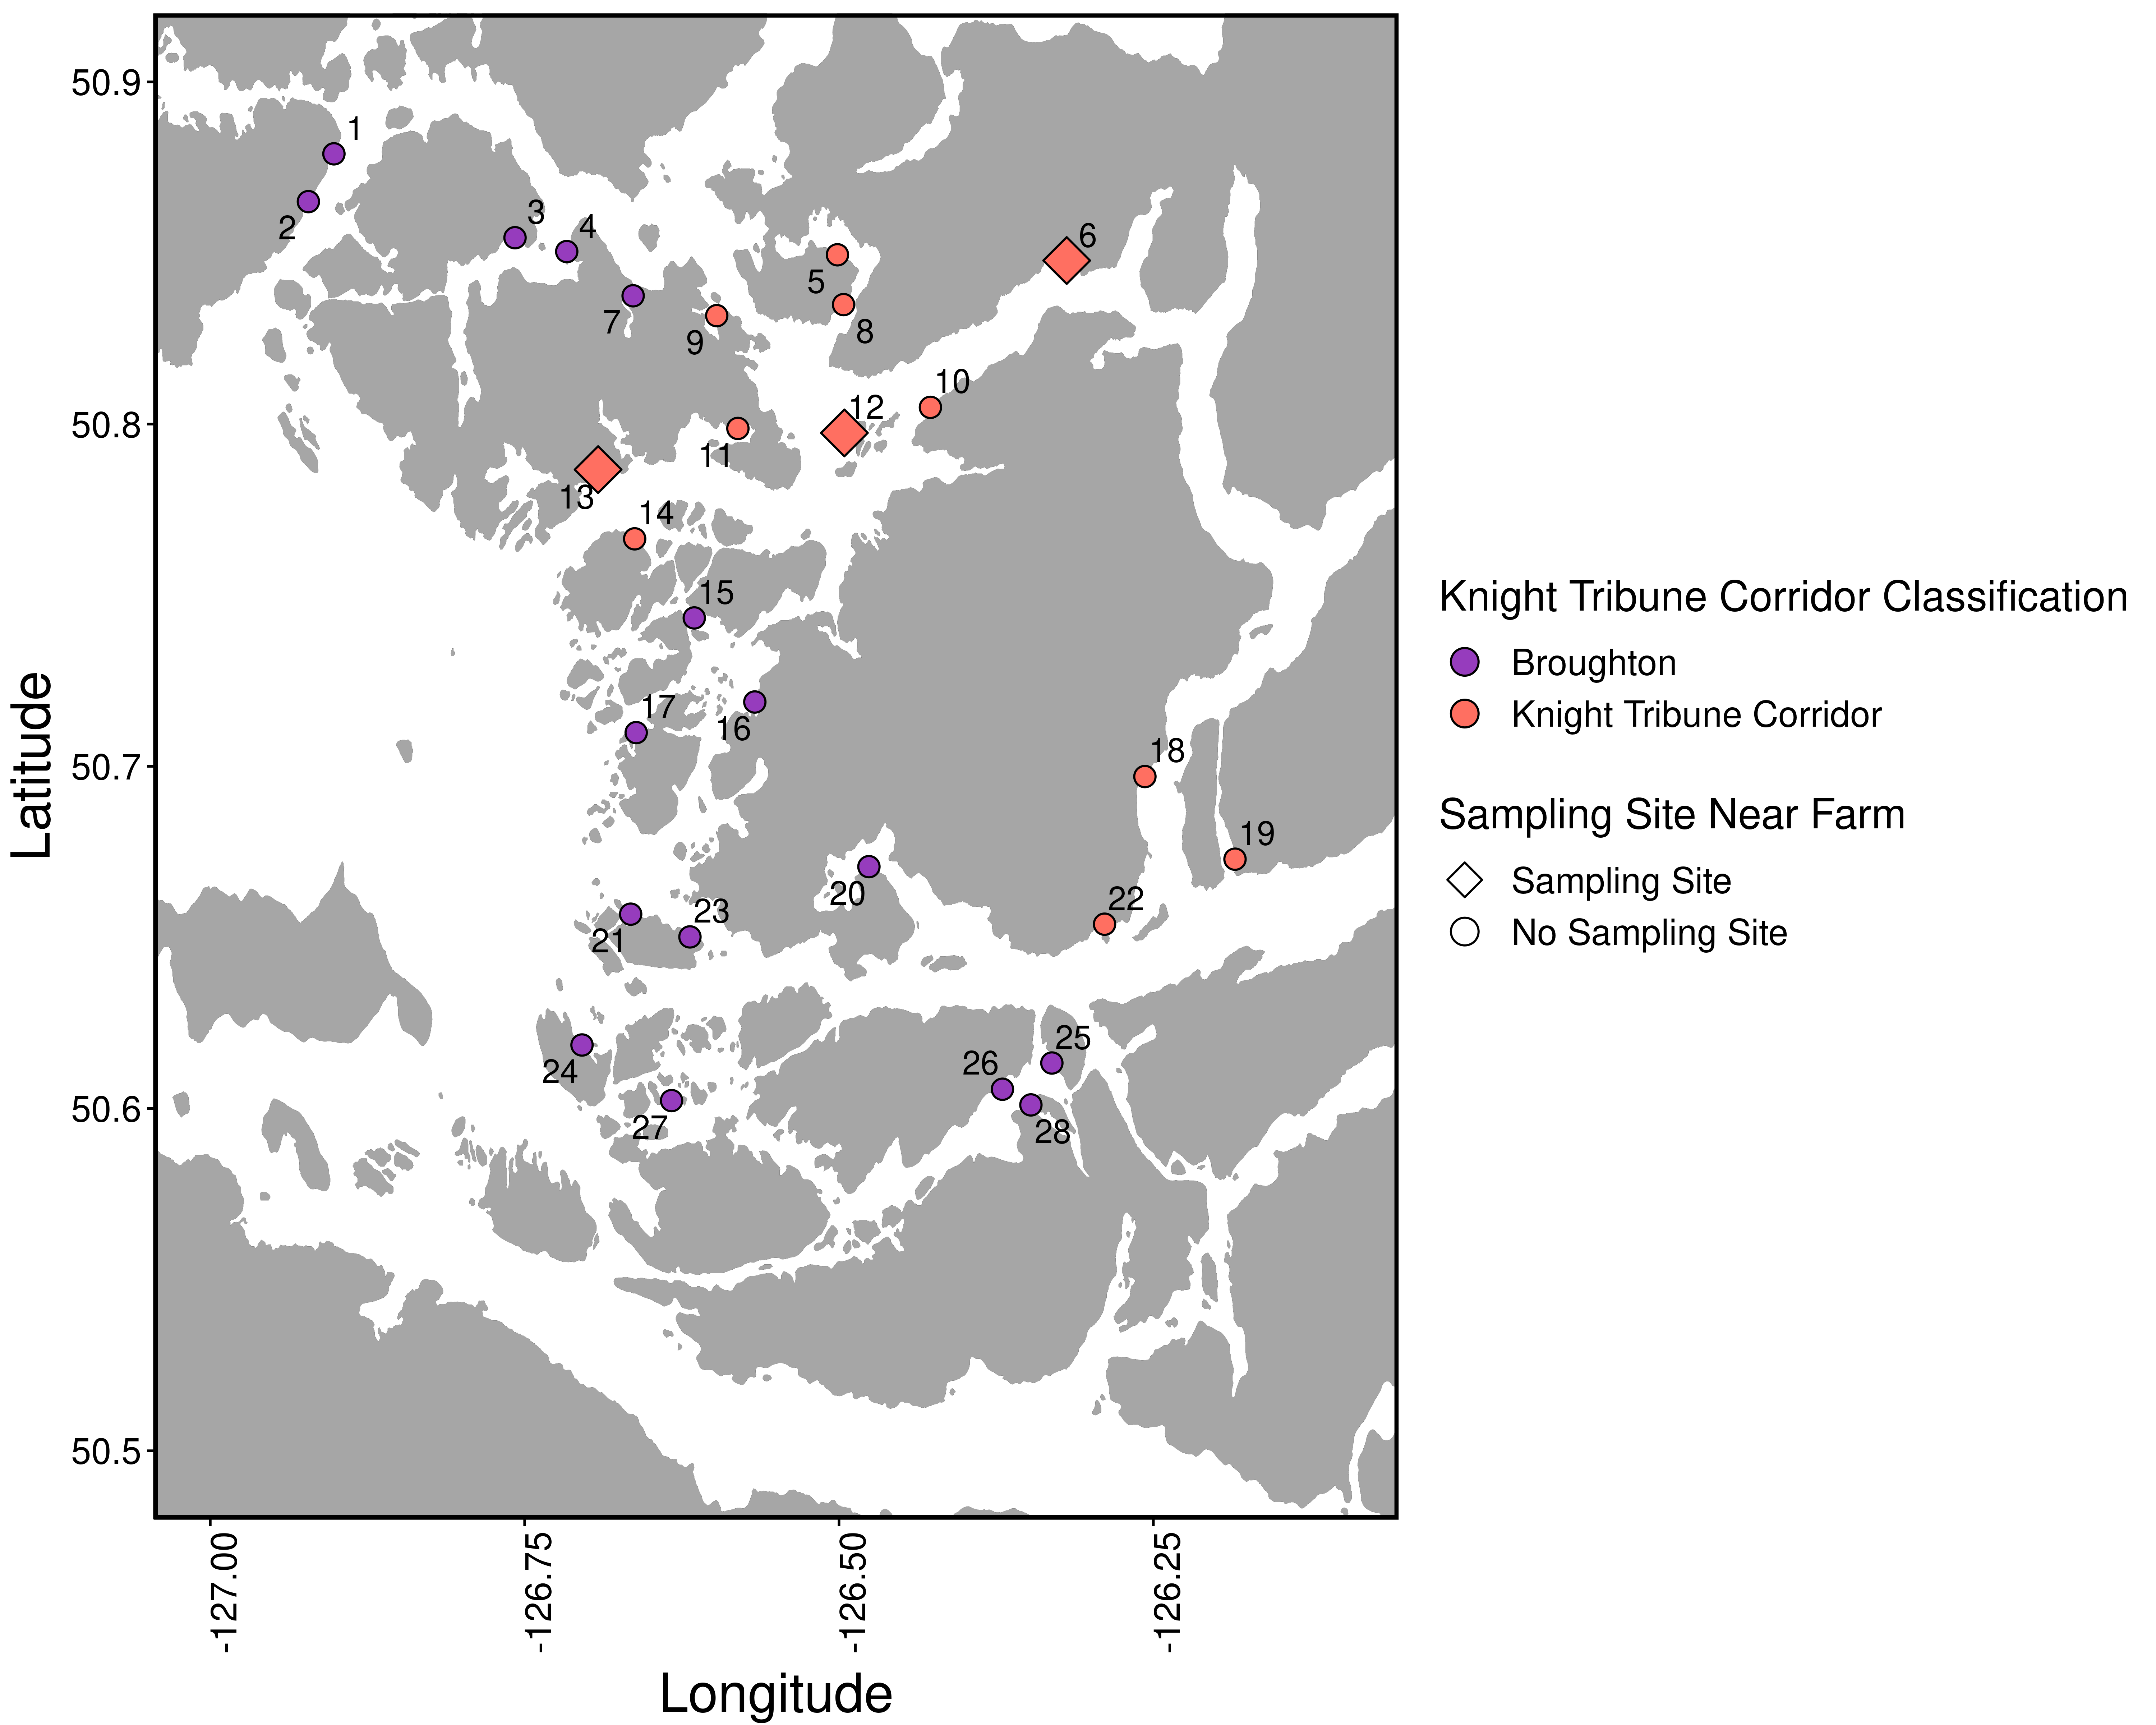
\includegraphics[width=\textwidth]{images/numbered-farm-map.png}
    \caption{Classification of the farms in the Broughton Archipelago. Labelled are the farmed in the Knight-Tribune corridor, as well as where the sampling points for wild juvenile salmon are. Note that in this map, the three focal farms - Humphrey, Sergeant, and Doctors are farms 18, 19, and 22 respectively.}
    \label{fig:map1}
\end{figure}

Given that some farms likely contribute more lice to the numbers infesting wild juvenile salmon, we compared three different groupings of the farms. We looked at the relationship of lice on wild juveniles to a) the number of lice on all farms, b) the number of lice on farms in the Knight-Tribune corridor, and c) the number of lice on three focal farms - Humphrey, Sergeant, and Doctors (Fig. \ref{fig:map1}). 

\subsection{Sea Lice on Wild Juvenile Salmon}

To account for sea lice on wild juvenile salmon, we used data collected from Salmon Coast Field Station that represents a long-term monitoring program, wherein juvenile pink salmon are sampled and examined for sea lice at weekly intervals from March to June between 2001 and 2021. Collection of these data are described in a variety of publications including (PUT ALL RELEVANT PAPERS HERE), but briefly, at the sampling sites, shoals of juvenile salmon were identified visually and then collected in a seine net. The juvenile salmon were then transferred to buckets, then either placed individually into sample bags and frozen for subsequent analysis (2001-2004), or analyzed non-lethally on size using a hand lens and visual assay. The lice counts we report here are the sum of all attached stages of \textit{L. salmonis}. 

In 2001, all attached lice identified were in the chalimus stage, but could not be identified to species level. To account for this, following the methods presented in Bateman et al. (2016), we estimate the proportion of chalimus that were \textit{L. salmonis} by regressing the proportion of \textit{L. salmonis} versus the number of total attached lice in other years, then predicting that proportion in 2001. Since the ratio of \textit{L. salmonis} to all lice increases asymptotically as the number of total lice increases, we use a nonlinear regression, which takes the form $$Y \sim a - (a - b)^{-cX}$$ where $a$ is the maximum attainable $Y$, $b$ is the value of $Y$ when $X$ is $0$ and $c$ is the proportional relative rate of the increase in $Y$ while $X$ increases. In our case, since $Y$ is continuous and bounded at $0$ and $1$, $a$ was given the value of $1.0$, $b$ is $0.0$ and $c$ is fit. 

This analysis indicates that the predicted proportion of \textit{L. salmonis} in 2001 is $>0.95$ (Fig. \ref{fig:lep-prop}.

\begin{figure}[h]
    \centering
    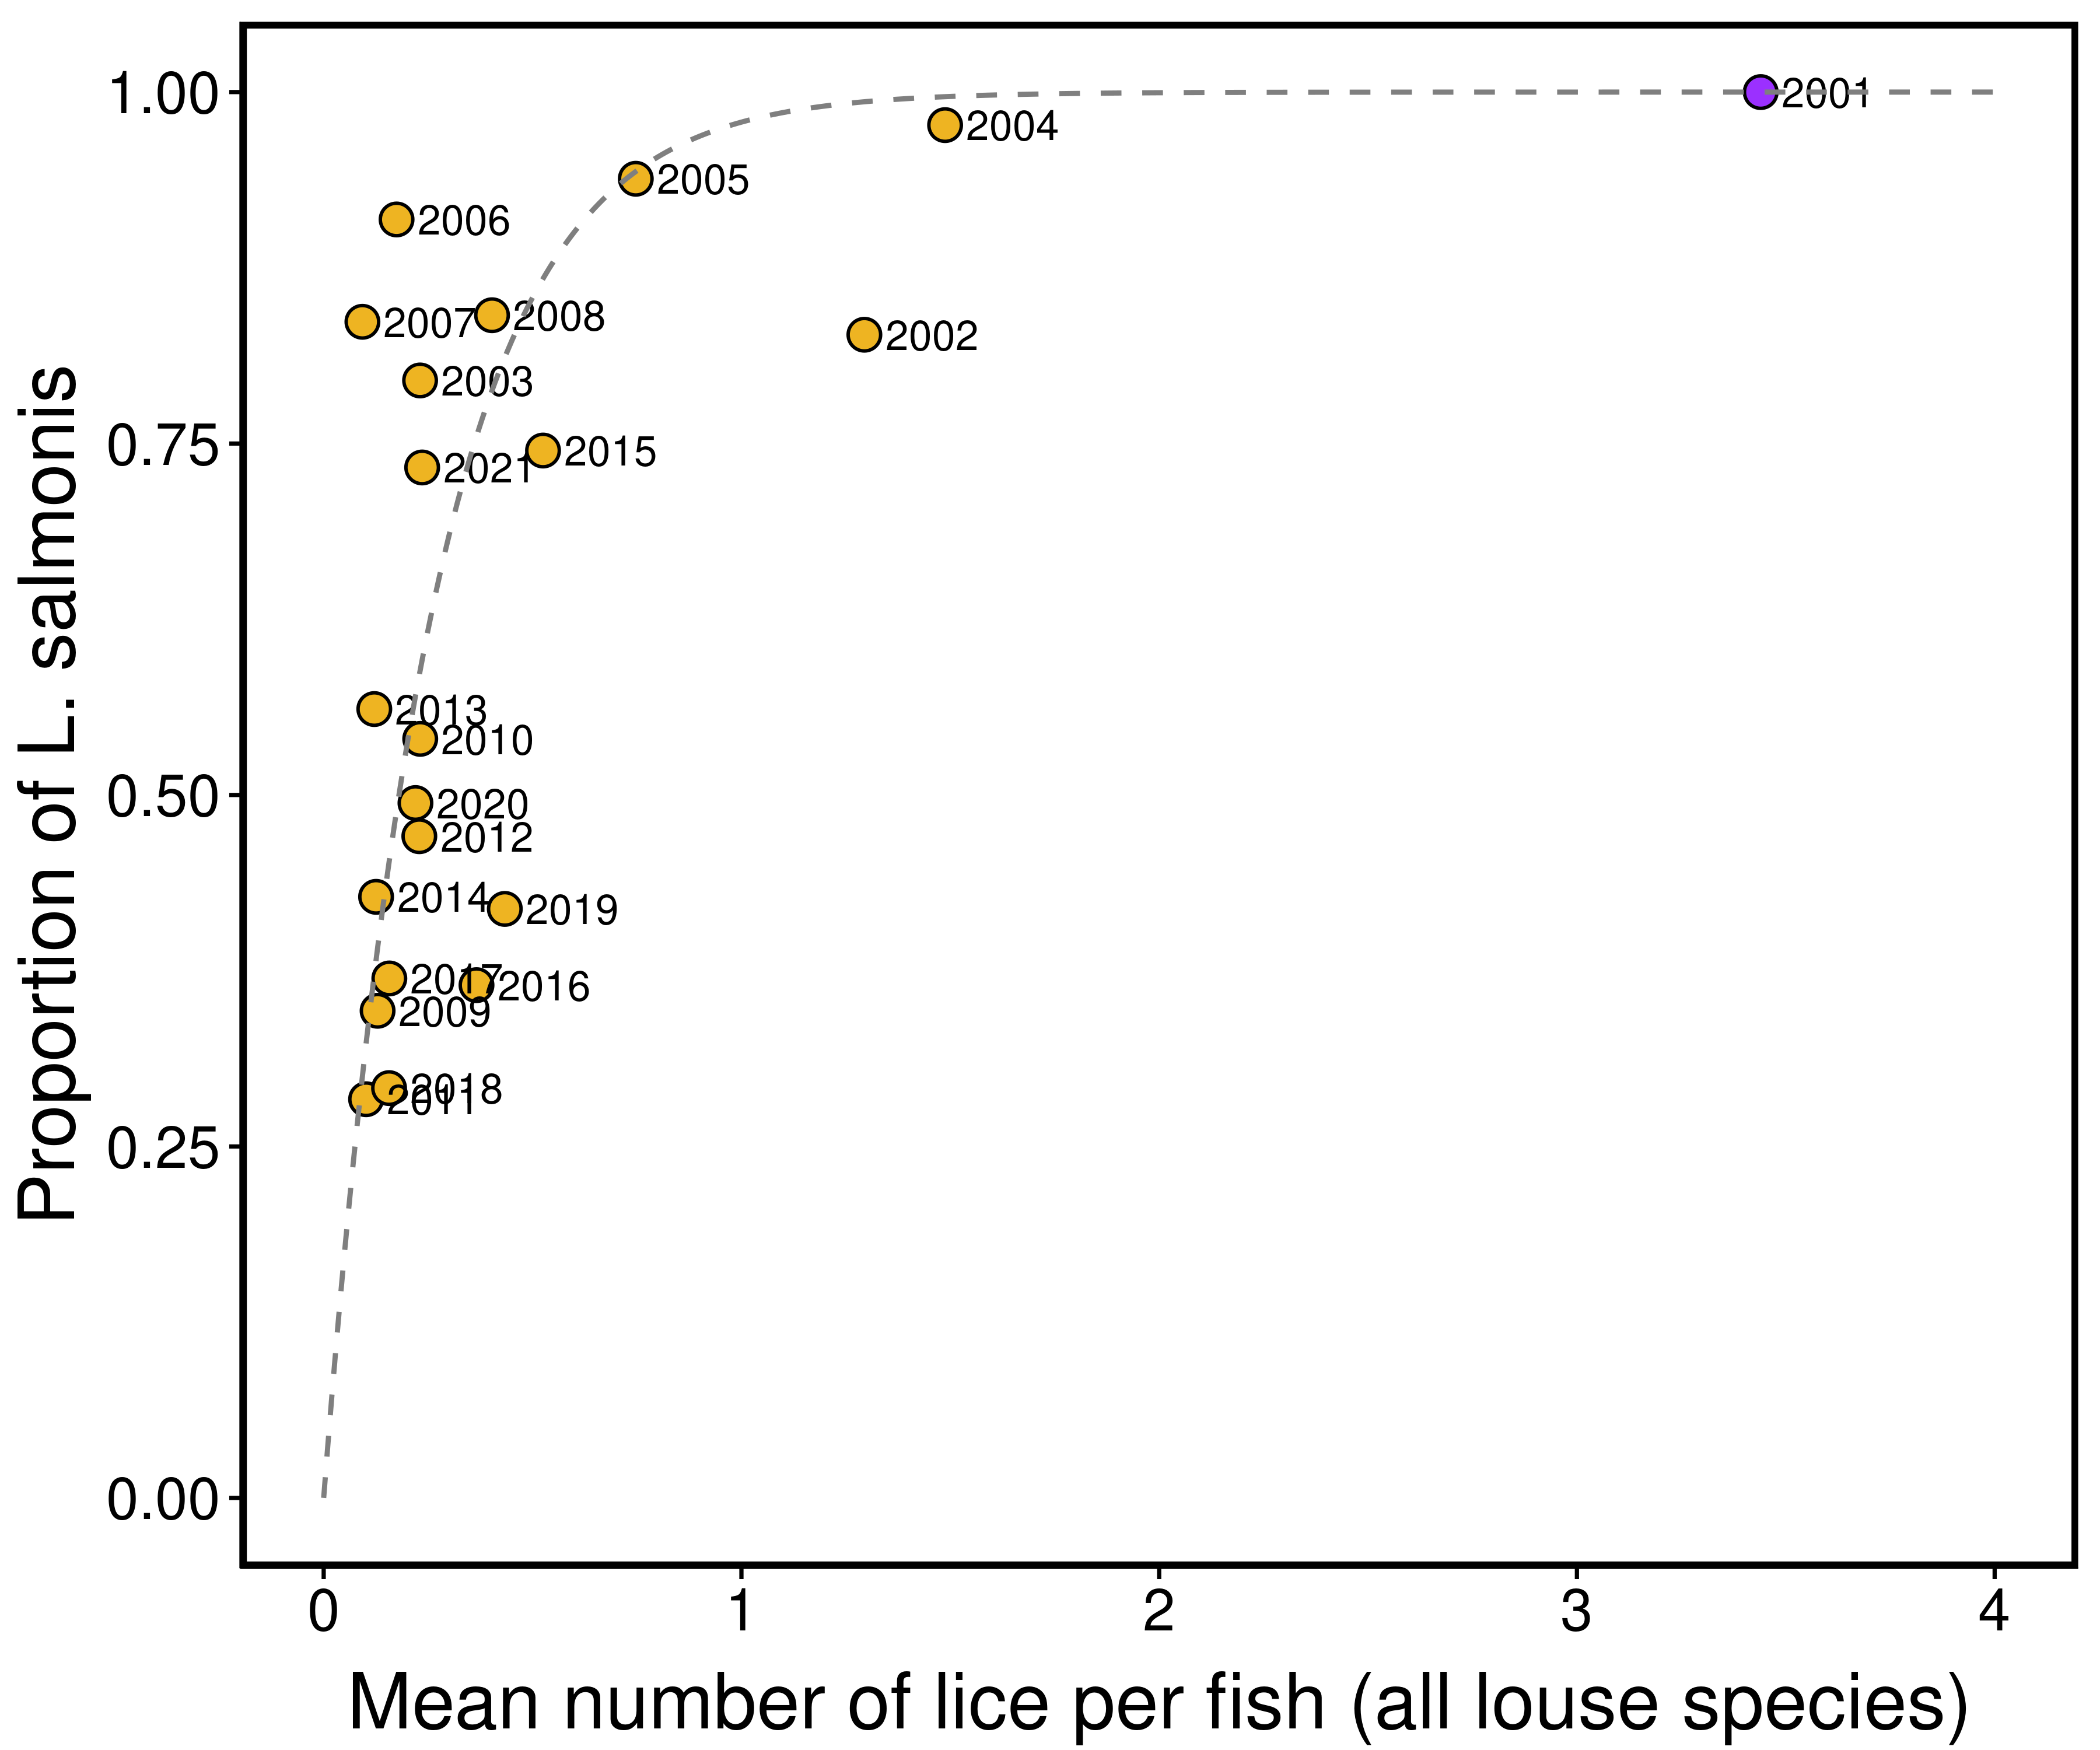
\includegraphics[width=\textwidth]{images/predicted-lep-proportions.png}
    \caption{Proportion of \textit{L. salmonis} relative to all species of lice. Yellow points represent data, the purple point represents a predicted value.}
    \label{fig:lep-prop}
\end{figure}

\subsection{Pink salmon spawner-recruit data}

\subsubsection{Spawner Abundance}

To understand the effect of lice on the returns and spawner abundance of pink salmon, we compared estimates of spawner abundance in the Broughton Archipelago to reference areas on the central coast (DFO fishery management areas 7-10). The data on spawner abundance were collected from the DFO New Salmon Escapement Database System (NuSEDS) which contain escapement data from 1956 to 2021, denoting separate rivers and even- vs odd-year populations. The methods of NuSEDS data collection have changed slightly through time, but are generally gathered by estimating spawner abundance via stream walks and overhead flights. 

\subsubsection{Recruitment Estimates}

Calculating recruitment follows the methodology laid out in Peacock (2013), but briefly, we summed the total estimated number of salmon removed from the stock via fisheries, with the spawner abundance (i.e. escapement) presented in the NuSEDS database. These catch estimates were obtained via two main sources. For Area 12 (Broughton Archipelago), we used data on run reconstructions provided by DFO, which were updated to the year 2021. For data for the other reference regions (Areas 7-10), we used estimates of exploitation rate and run size from English et al. (2018), which include data up to 2017. 

When estimating escapement, we calculate that rate for each year and area as $$\mu_{i,t} = \frac{C_{a,t}}{C_{a,t} + E_{a,t}}$$ where exploitation rate $u_{i,t}$ is given for each river $i$ and each year $t$, as the proportion of the catch $C_{a,t}$ in each area $a$ and year $t$ relative to the sum of all estimated escapement $E$ and catch $C$. Note that this assumes all rivers $i$ within fishery management areas $a$ to have the same exploitation rate in a given year $t$.

With this information we can then estimate the amount of recruitment, $R_{i,t}$ to each river $i$ in each year $t$ as $$R_{i,t} = \frac{N_{i,t}}{1 - u{i,t}},$$ where $N_{i,t}$ is the spawner abundance of pink salmon from year $i$ in year $t$, and $u_{i,t}$ is the exploitation rate for river $i$ in year $t$. 

When performing the analysis, we compared two methods of screening river-year combinations for sufficient data. In the main analysis presented here, we use a dataset where we screened out populations that had $<4$ stock-recruit pairs, in accordance with previous work. This yielded a data set with 78 rivers, and a total of 2744 stock-recruit pairs across 149 populations (even/odd). Note that the number of rivers sampled in each year through time was not consistent (Fig. \ref{fig:cutof-comp})

\begin{figure}[h]
    \centering
    \makebox[\textwidth][c]{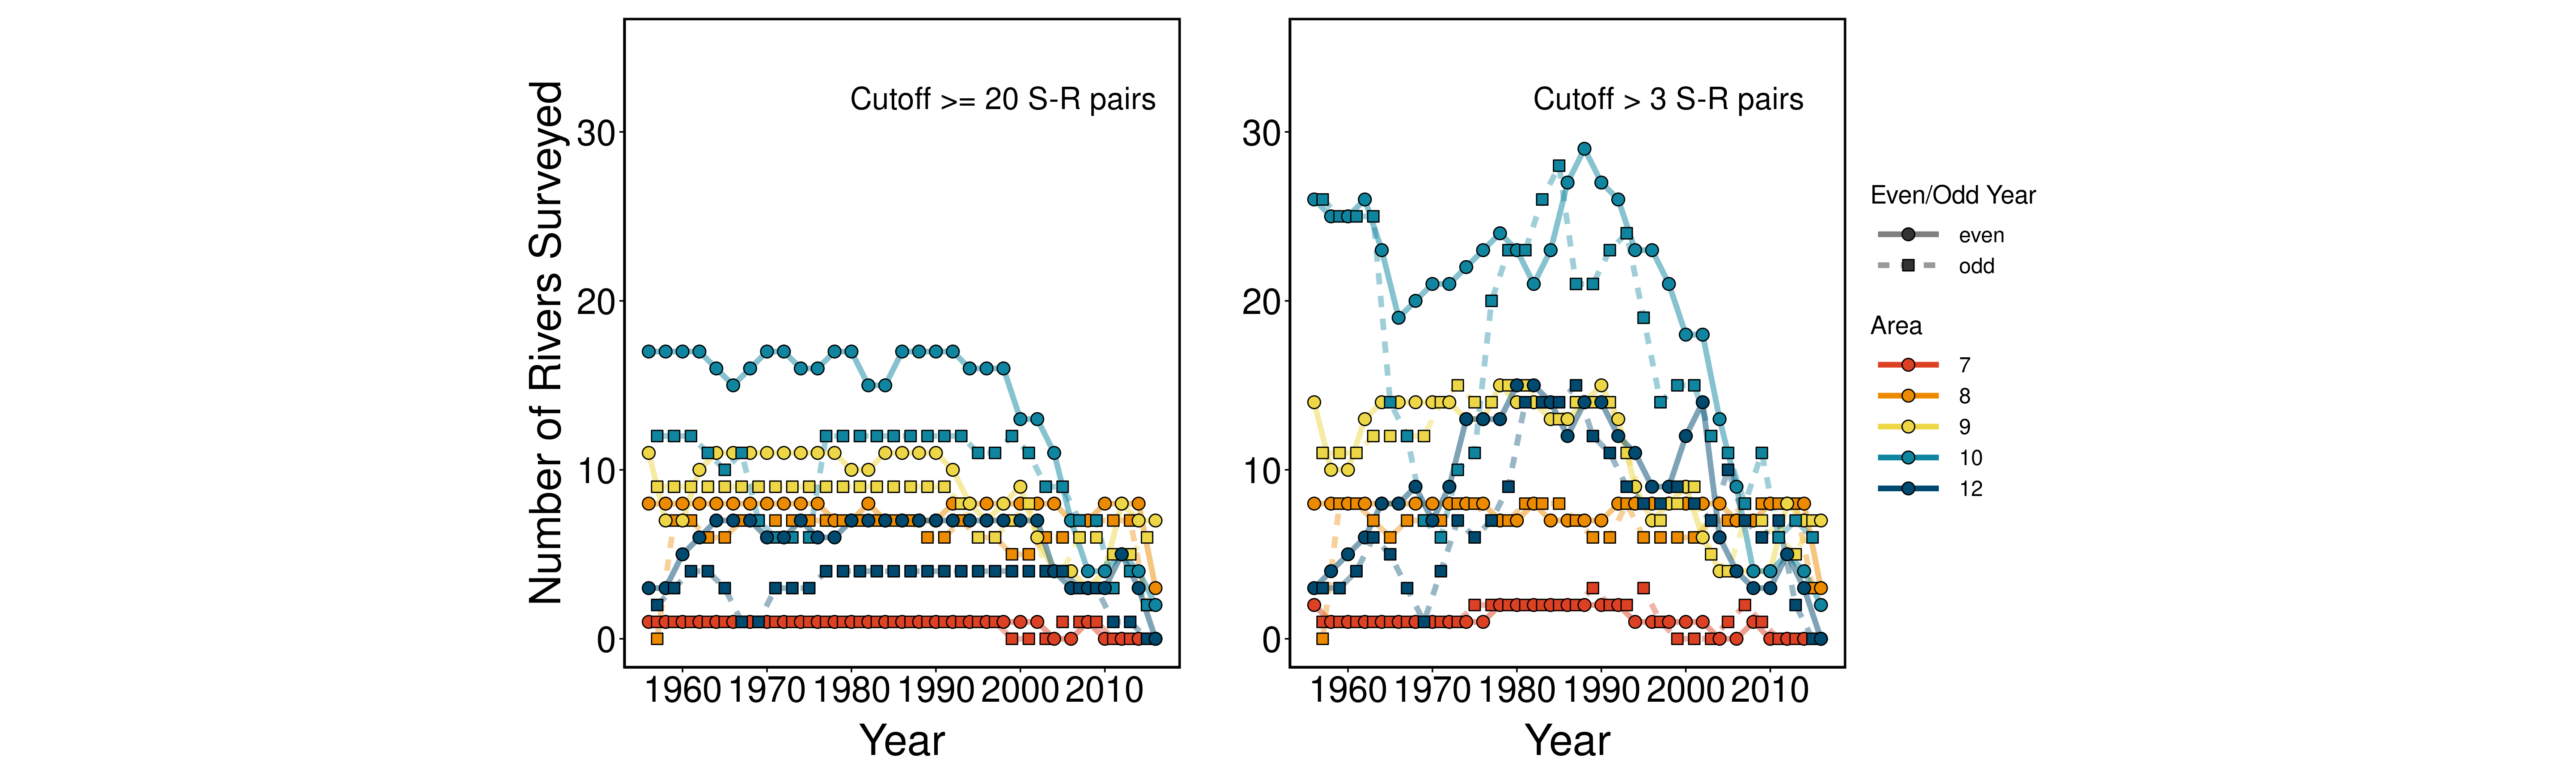
\includegraphics[width=2.1\textwidth]{images/rivers-surveyed-through-time-comparison.png}}%
    \caption{Number of rivers in each year and each area that were surveyed by DFO to enumerate the number of spawners.}
    \label{fig:cutof-comp}
\end{figure} 

\subsection{Relationship Between Farm Lice \& Wild Juvenile Lice}

In order to estimate the effect of lice on the returns of pink salmon, we needed to make estimates of the mean number of \textit{L. salmonis} per wild juvenile salmon in each year, via data from weekly monitoring surveys in the years 2001-2021. We estimated the mean number of lice per year with a generalized linear mixed-effects model (GLMM) where year was a fixed effect and both sample site (Fig. \ref{fig:map1}) and week were random effects. We then compared the number of lice on wild juveniles to the number of lice on salmon farms in the region. To do this, we compared three different groupings of salmon farms. We looked at the relationship of lice on wild juveniles to a) the number of lice on all farms, b) the number of lice on the farms in the Knight-Tribune corridor (KTC) (Fig. \ref{fig:map1}), and c) the number of lice on three focal farms - Humphrey, Seargeant, and Doctors. This analysis was done using the glmmTMB package (CITE). 

A preliminary regression analysis revealed that the number of lice on both a) all farms, and b) KTC farms explained the number of lice on wild lice well (Fig. \ref{fig:farm-comp}). While both the "All Farms" and KTC groupings provided high correlation with lice on wild juveniles ($R^2$ = 0.77 \& 0.72 respectively), we show that the number of lice on wild juveniles is best predicted by the number of lice on all farms. 

\begin{figure}[h]
    \centering
    \makebox[\textwidth][c]{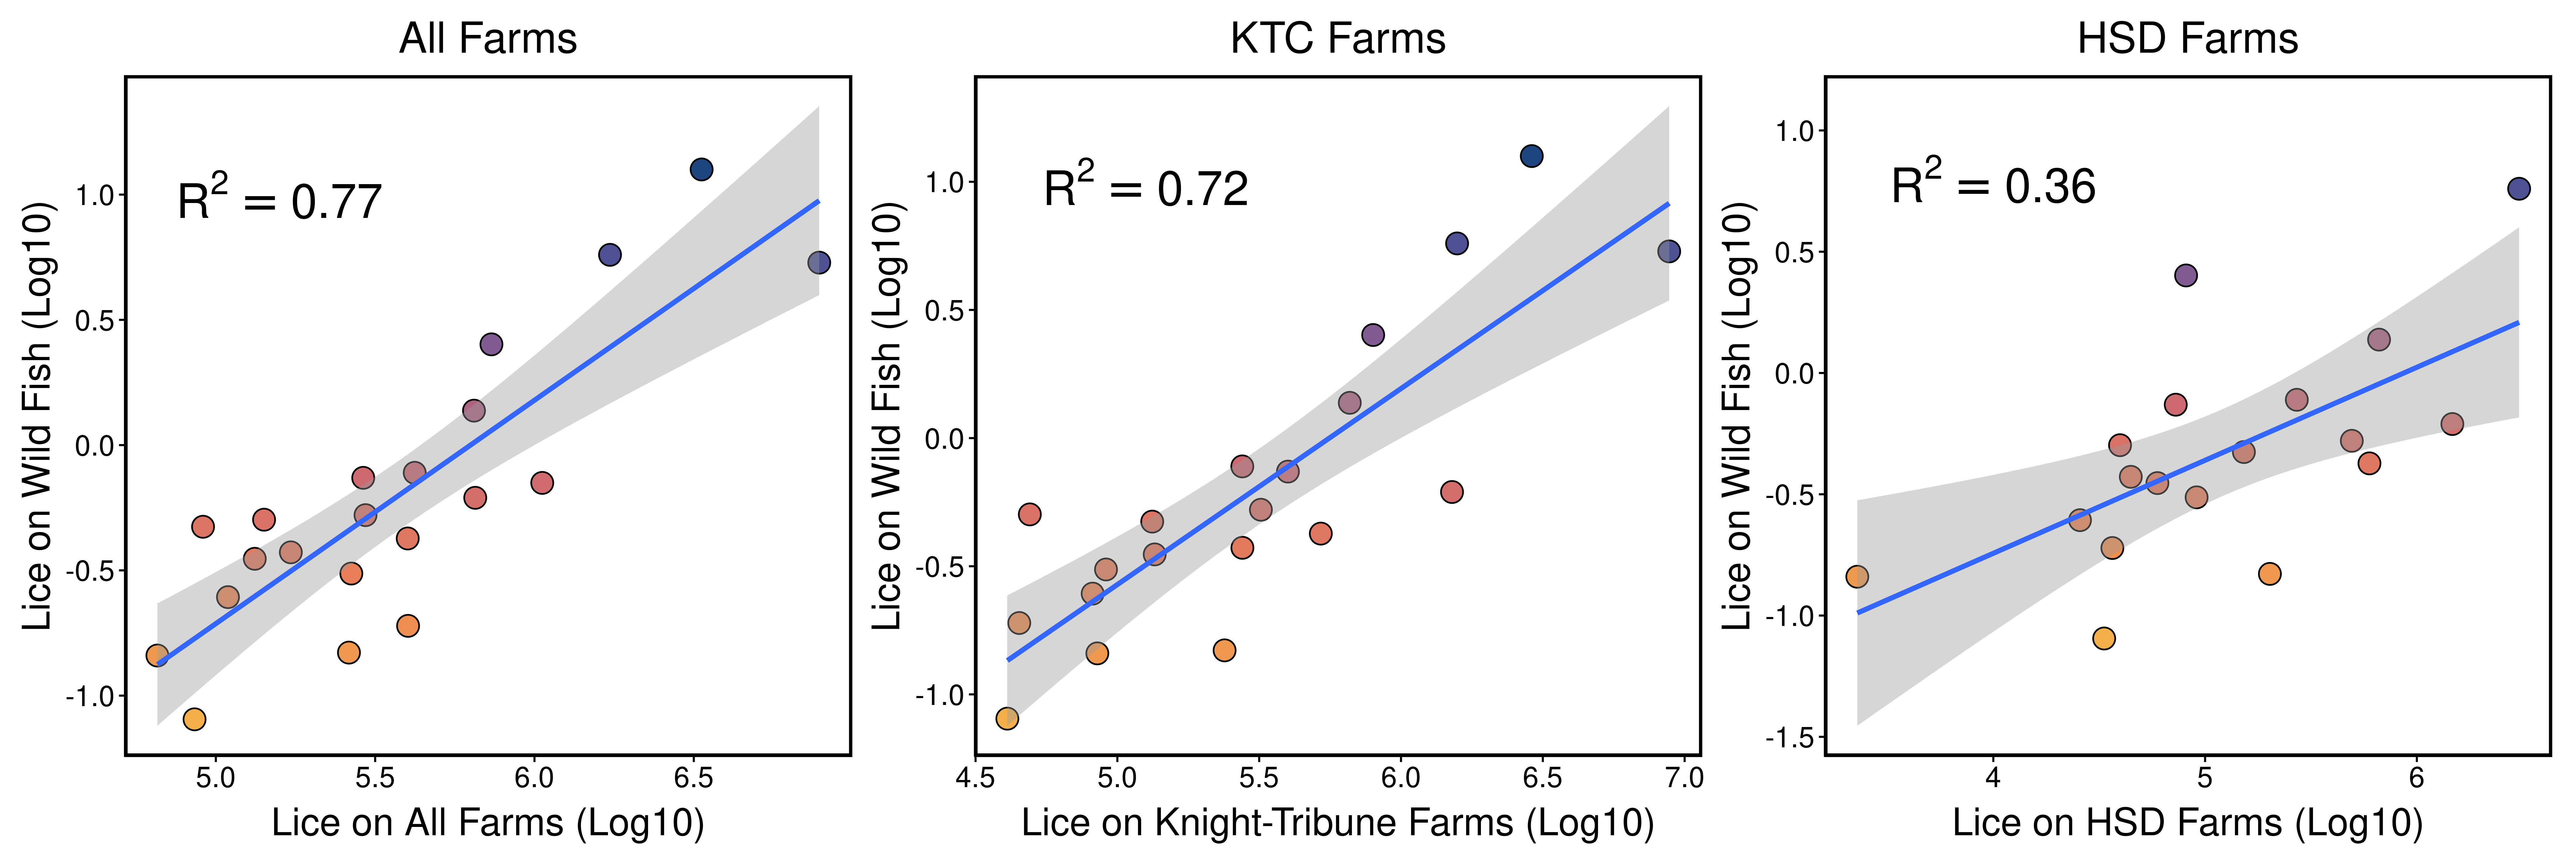
\includegraphics[width=1.3\textwidth]{images/wild-to-farm-models-comparison.png}}%
    \caption{A comparison of the relationship between the number of lice on
wild salmon (on a $log_{10}$ scale), and the number of lice on the three sets of farm
comparisons (also a $log_{10}$ scale).}
    \label{fig:farm-comp}
\end{figure} 

\subsection{Model Analysis}

To directly model the effect of sea lice on the survival of pink salmon populations, we used a hierarchical version of the classic Ricker model (Ricker 1954), described in Peacock et al. (2013). This approach allowed us to treat populations in the Broughton region (area 12) as being exposed to salmon farms while populations in other regions (7-10) were not exposed to local salmon farms. 

The hierarchical Ricker model can be described as $$R_{i,t} = N_{i,t-2} \textrm{ exp} \left[r-b_i N_{i,t-2} -c W_{a,t-1} + \theta_{t} + \theta_{a,t} + \varepsilon_{i,t}\right]$$ where $R_{i,t}$ is the number of recruits to population $i$ in year $t$,  $N_{i,t-2}$ is the number of spawners in population $i$ at year $t-2$. This $t$ lag is to account for the two-year lifespan of pink salmon. $r$ is the growth rate which is treated as singular across different populations, but $b_i$ is the density-dependence parameter which is unique to each population, to represent the different habitat factors and competitive interactions each population $i$ experiences independently. Further, the term $cW_{a, t-1}$ is the modelled effect of sea lice from salmon farms on the juvenile pink salmon. Here, $W_{a, t-1}$ is the number of sea lice in each area $a$ in time $t-1$. We assume the number of lice in areas 7-10 to be zero since there are no salmon farms in that region, and the mean number of lice per juvenile salmon per year in area 12, is estimated from the GLMM described previously. Thus, since $W_{a, t-1}$ are data in this formulation, we fit $c$ as the coefficient, giving the direct estimated percent mortality of pink salmon due to sea lice on wild juvenile salmon equal to $1-\textrm{exp}(-cW_{a,t-1})$ (Krkosek et al. 2011; Peacock et al. 2013). 

With respect to data on sea lice, no measurements of lice on wild juvenile salmon exist pre-2001, so in line with Peacock et al. (2013), we assume that $W_{a,t-1}$ are "missing" data from 1991-2001, and pre-1991 are 0.

We account for three forms of stochasticity in this analysis. First, the environmental stochasticity which varies through time but is consistent in time $t$ for all populations. This is modeled as $\theta_t$, a normally distributed random variable with a mean of zero and an estimated variance. Second, we account for environmental stochasticity which varies through time $t$ and between areas $a$, such that all populations within an area $a$ are subject to the same effect. This is $\theta_{a,t}$, a normally distributed random variable with a mean of zero and an estimated variance. Last, we also account for environmental stochasticity that varies through years $t$ and between populations $i$. This is $\varepsilon_{i,t}$, a normally distributed random variable with mean zero and estimated variance. 

As in Peacock (2013), we fit the Ricker model in a linear form $$\textrm{ln}\frac{R_{i,t}}{N_{i,t-2}} = r - b_i N_{i,t-2} - c W_{a,t-1} + \theta_t + \theta_{a,t} + \varepsilon_{i,t}$$ in the lme4 package. We compared the fit of this model to a null model version without any term accounting for effects from sea lice. To estimate variance around our maximum likelihood estimates, we calculated confidence intervals on our model parameters via parametric bootstrapping, described in detail in (Marty paper 2007 \& 2012). 

To predict the \% mortality in future years, we used the predicted mean number of lice on juvenile salmon from our GLMM as our values for $W_{a,t-1}$, along with our fitted value for $c$. To get some measure of variance, we also took the 2.5th and 97.5th percentile values from the confidence interval of the GLMM predictions, and used those values for our values of $W_{a,t-1}$ to predict an upper and lower bound. 

All analysis presented here was performed in the R statistical computing language (R Core Team 2022). 

\section{Results}

Corroborating previous analyses of the first $\sim$half of these data, we note that the number of sea lice per wild juvenile salmon in the Broughton region declined from 2001 when surveys started, with an increase in 2015 (Fig. \ref{fig:wild-lice}). We note that the patterns of farmed salmon inventory over the past $\sim 20$ years has been sporadic (Fig. \ref{fig:timeseries}, but relatively consistent, whereas the number of lice on farmed salmon has a series of peaks and declines. Evidently for both values there is a substantial increase since January of 2020.  

\begin{figure}[h]
    \centering
    \makebox[\textwidth][c]{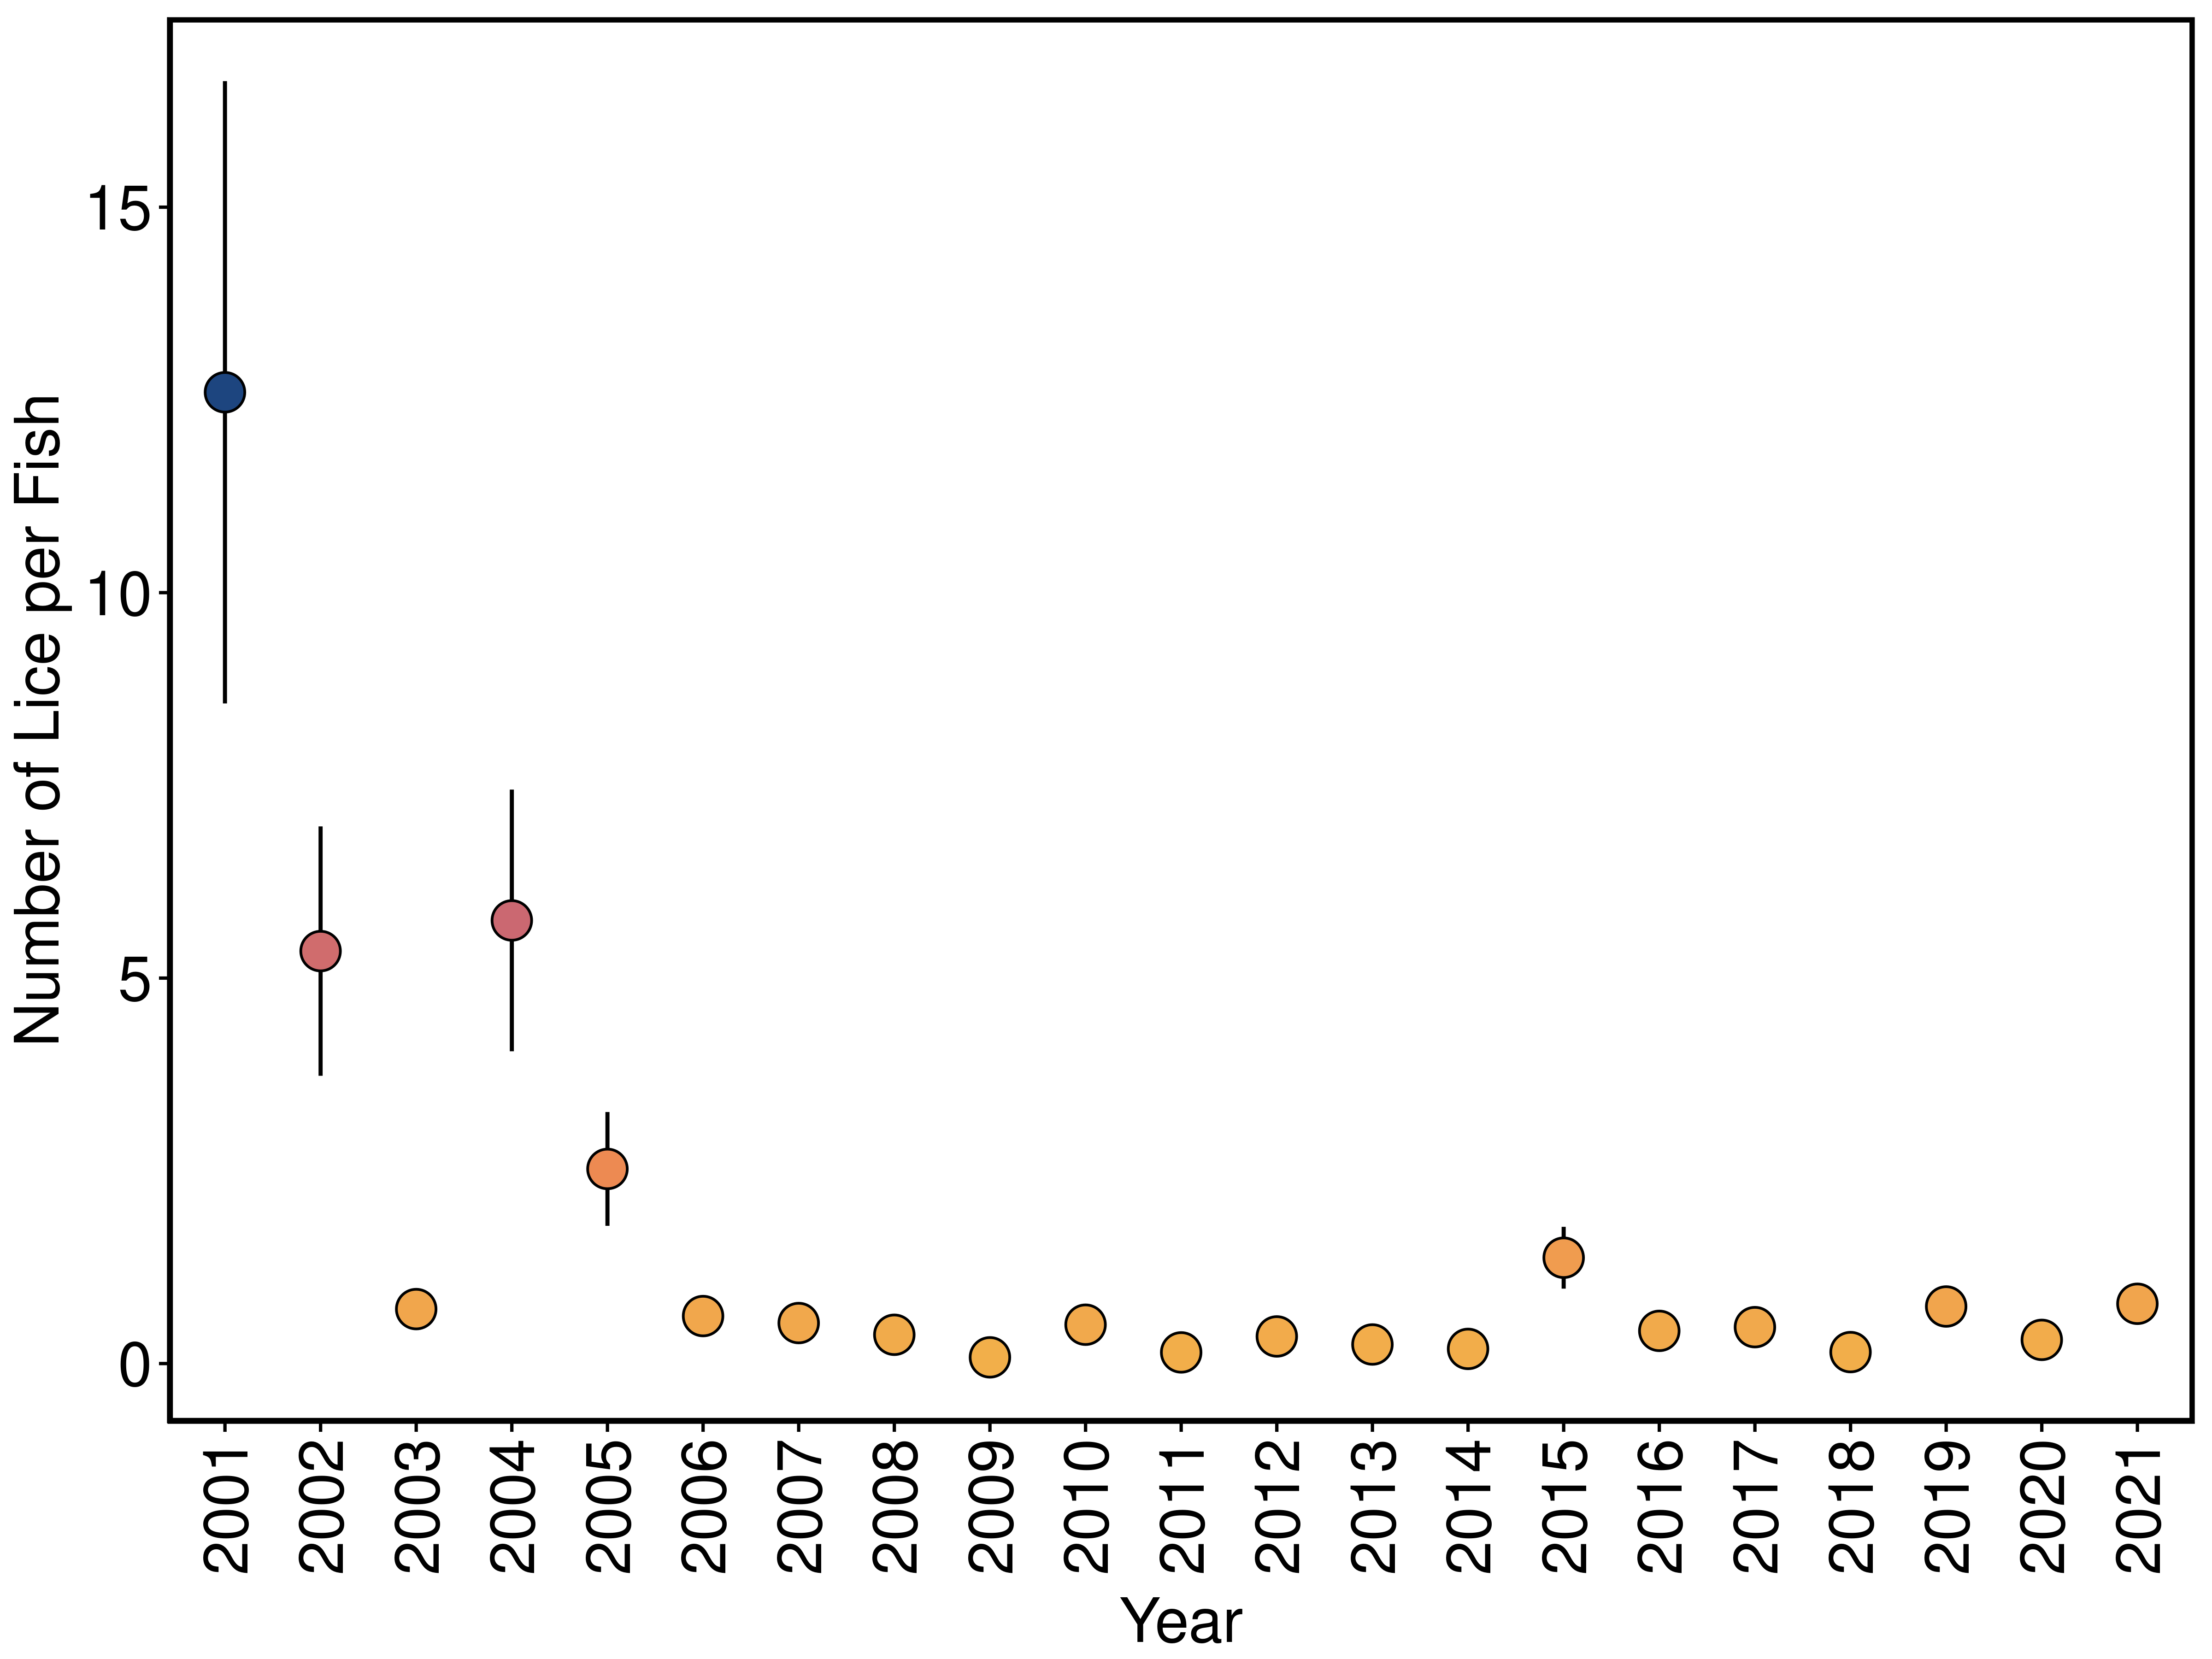
\includegraphics[width=1.0\textwidth]{images/just-wild-raw-comparison.png}}%
    \caption{Estimated number of lice per wild juvenile pink salmon in all available years. The points represent the estimated value, with the error bars giving a 95\% confidence interval.}
    \label{fig:wild-lice}
\end{figure} 

\begin{figure}[h]
    \centering
    \makebox[\textwidth][c]{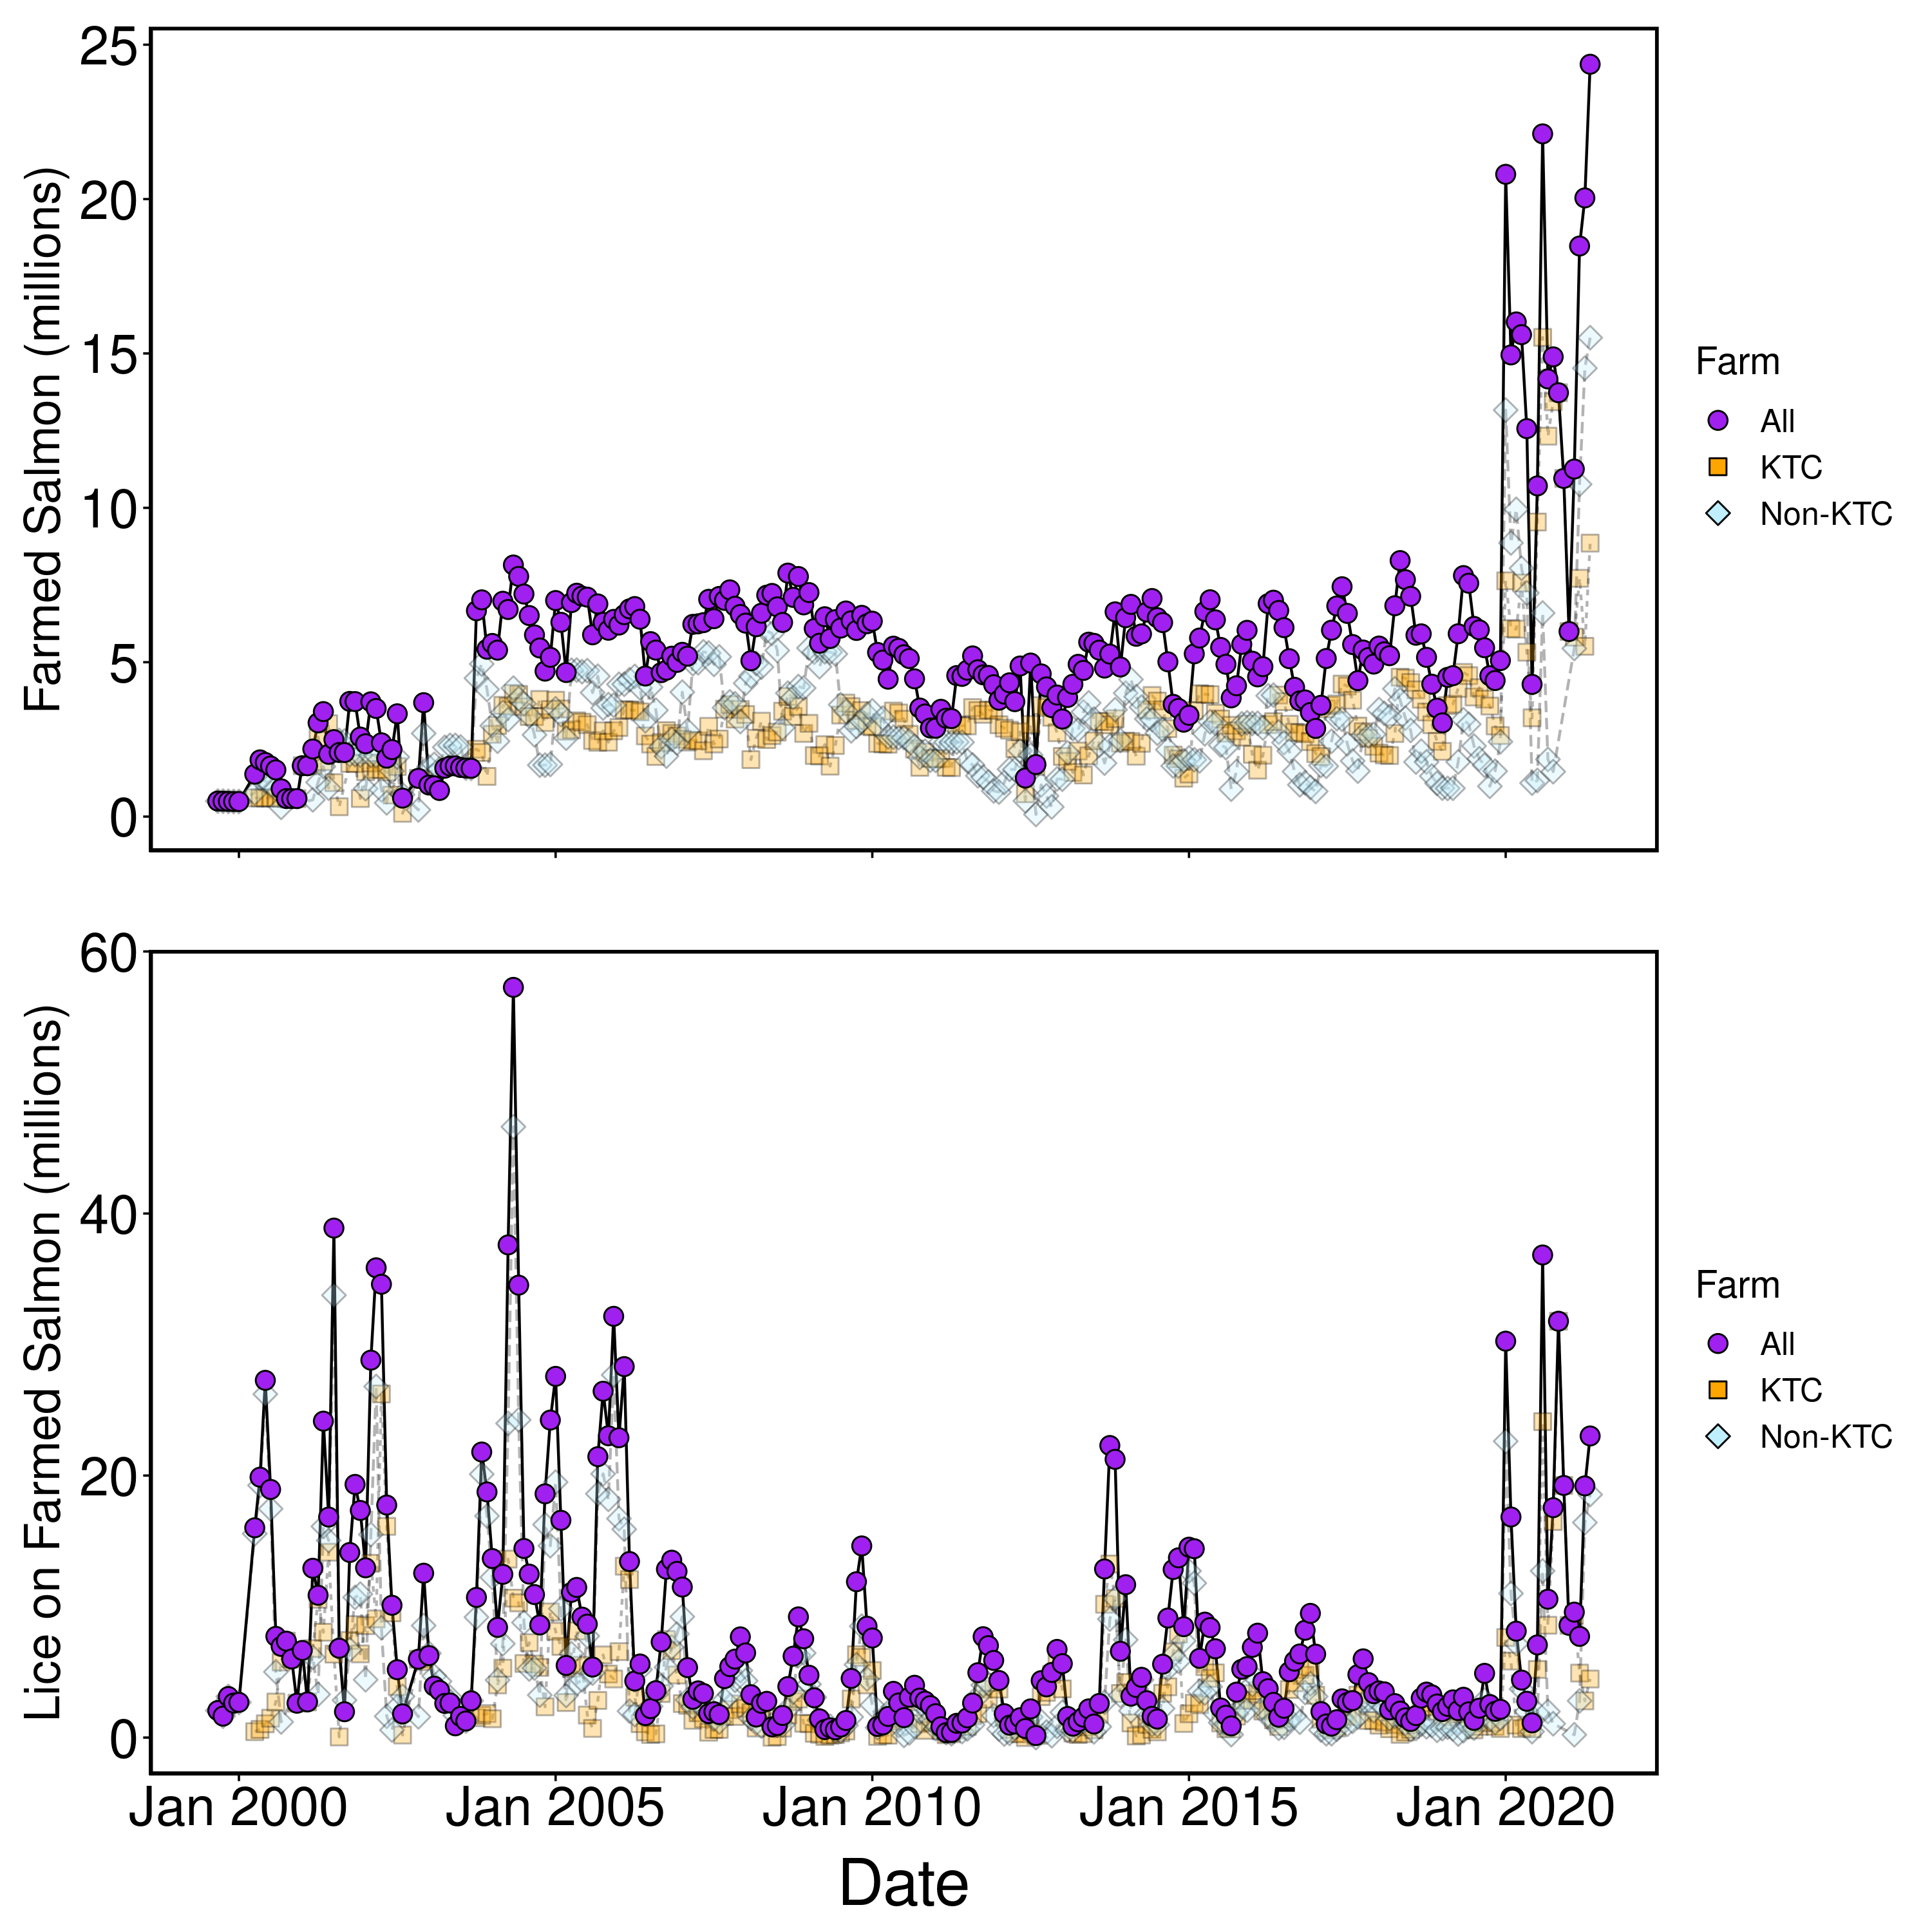
\includegraphics[width=1.4\textwidth]{images/fish-and-lice-on-farms-timeseries.png}}%
    \caption{Number of farmed salmon and the number of lice on those salmon, summed across farms in each month. Farms are divided into Knight-Tribune Corridor (KTC) farms, non-KTC farms, and the sum of those two values - "All".}
    \label{fig:timeseries}
\end{figure} 

When comparing our null model, which did not have any term accounting for sea lice, with our alternate model, we found the alternate model which included the term $c W_{a,t-1}$, outperformed the null model significantly (Table. \ref{table:1}). 

\begin{table}[h!]
\centering
\begin{tabular}{|c c c c c|} 
 \hline
 \textbf{Model} & \textbf{AIC} & \textbf{Neg. Log-Likelihood} & \textbf{Deviance} & \textbf{$\Delta$AIC} \\ [0.5ex] 
 \hline
  Alternative Model & 8909.5 & -4300.8 & 8601.5 & 0\\ 
  Null Model & 8927.9 & -4311.0 & 8621.9 &  18.4\\ [1ex] 
 \hline
\end{tabular}
\caption{Model comparison for null model and alternative model assessing if including a term for lice infestation improved fit of model of survival.}
\label{table:1}
\end{table}

Our two key parameters we were interested in from the Ricker model were $r$ the growth rate, and $c$ the effect of lice. We estimated $r$ to be 1.04 (95\% CI: 0.86, 1.23) and $c$ to be -0.24 (95\%CI: -0.34, -0.13). In our estimation of the the mean number of lice on wild juvenile salmon, we show that the average estimated percent mortality of pink salmon due to sea lice on wild juvenile salmon has generally declined since the beginning of the outbreak in the late 1990s/early 2000s (Fig. \ref{fig:est-mort} \& \ref{fig:surv}). 

\begin{figure}[h]
    \centering
    \makebox[\textwidth][c]{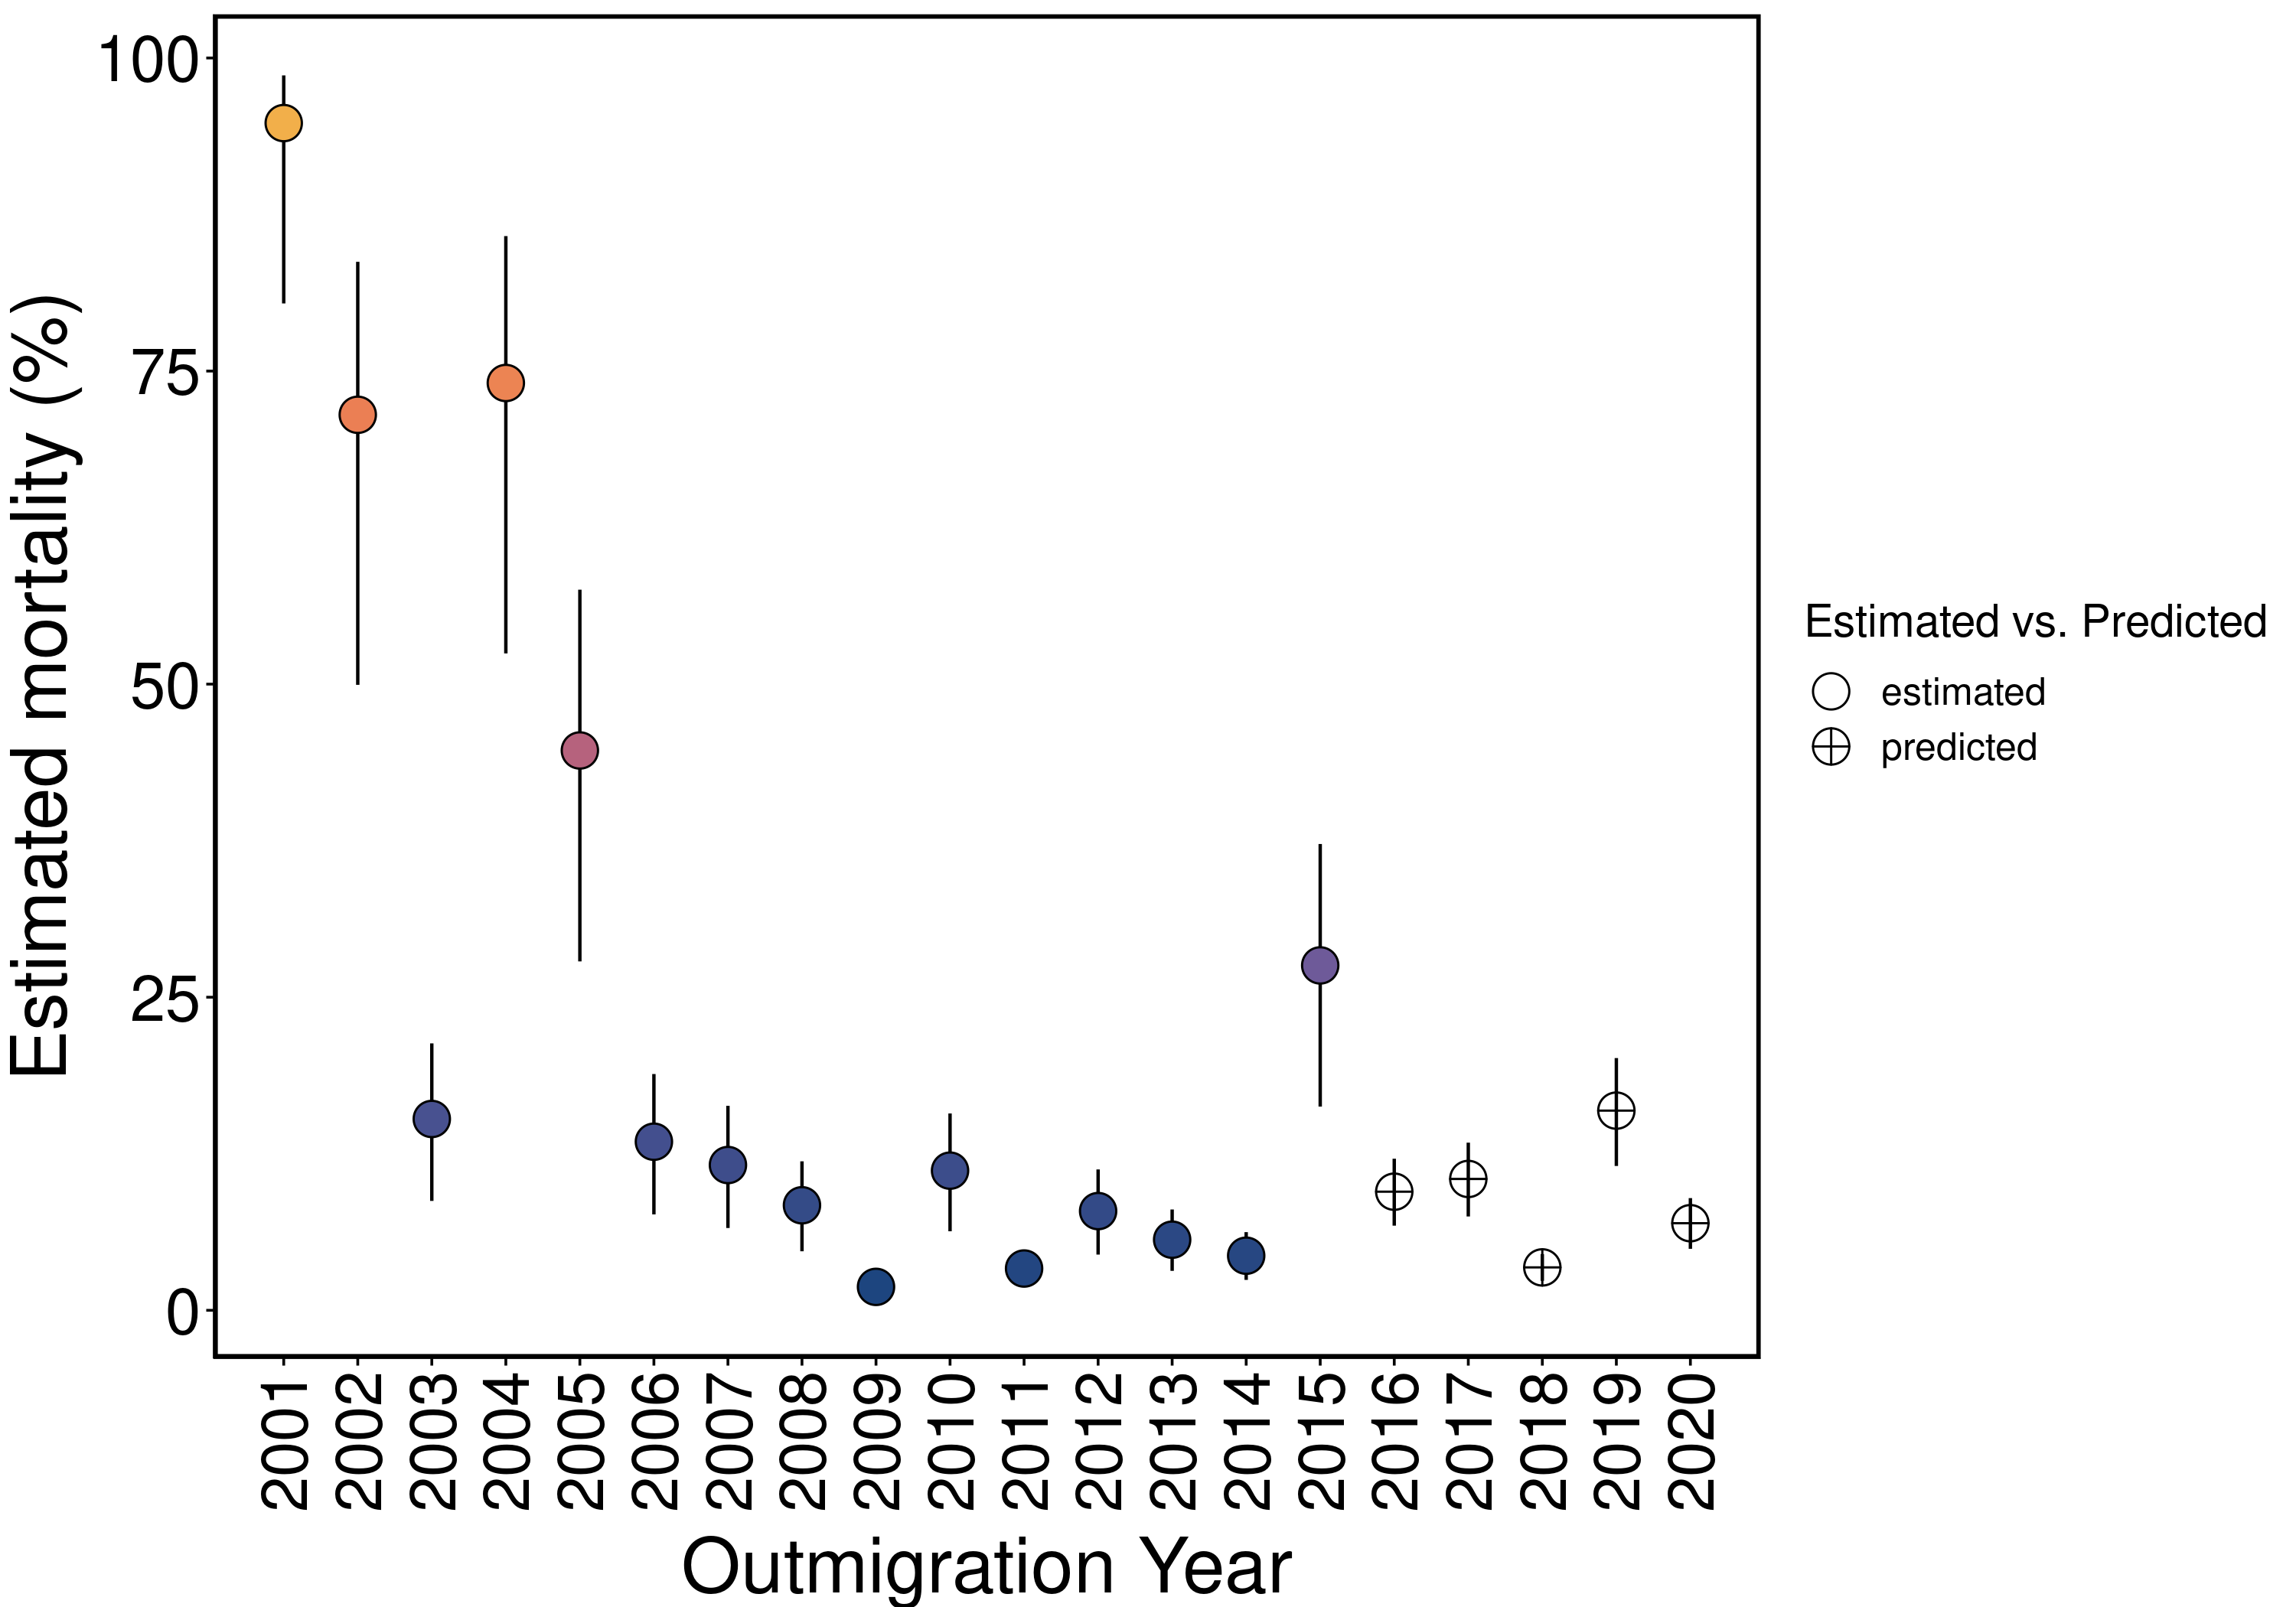
\includegraphics[width=1.4\textwidth]{images/estimated-mortality.png}}%
    \caption{Estimated and predicted percentage of the mortality in a given outmigration year, due to sea lice infestations of juvenile salmon $1-\textrm{exp}(-cW_{a,t-1})$. The points for the estimated values represent maximum likelihood estimates, and the error bars are 95\% confidence intervals. The error bars on the predicted values are not \textit{true} 95\% CI's, but are a best-estimate of those bounds.}
    \label{fig:est-mort}
\end{figure} 

\begin{figure}[h]
    \centering
    \makebox[\textwidth][c]{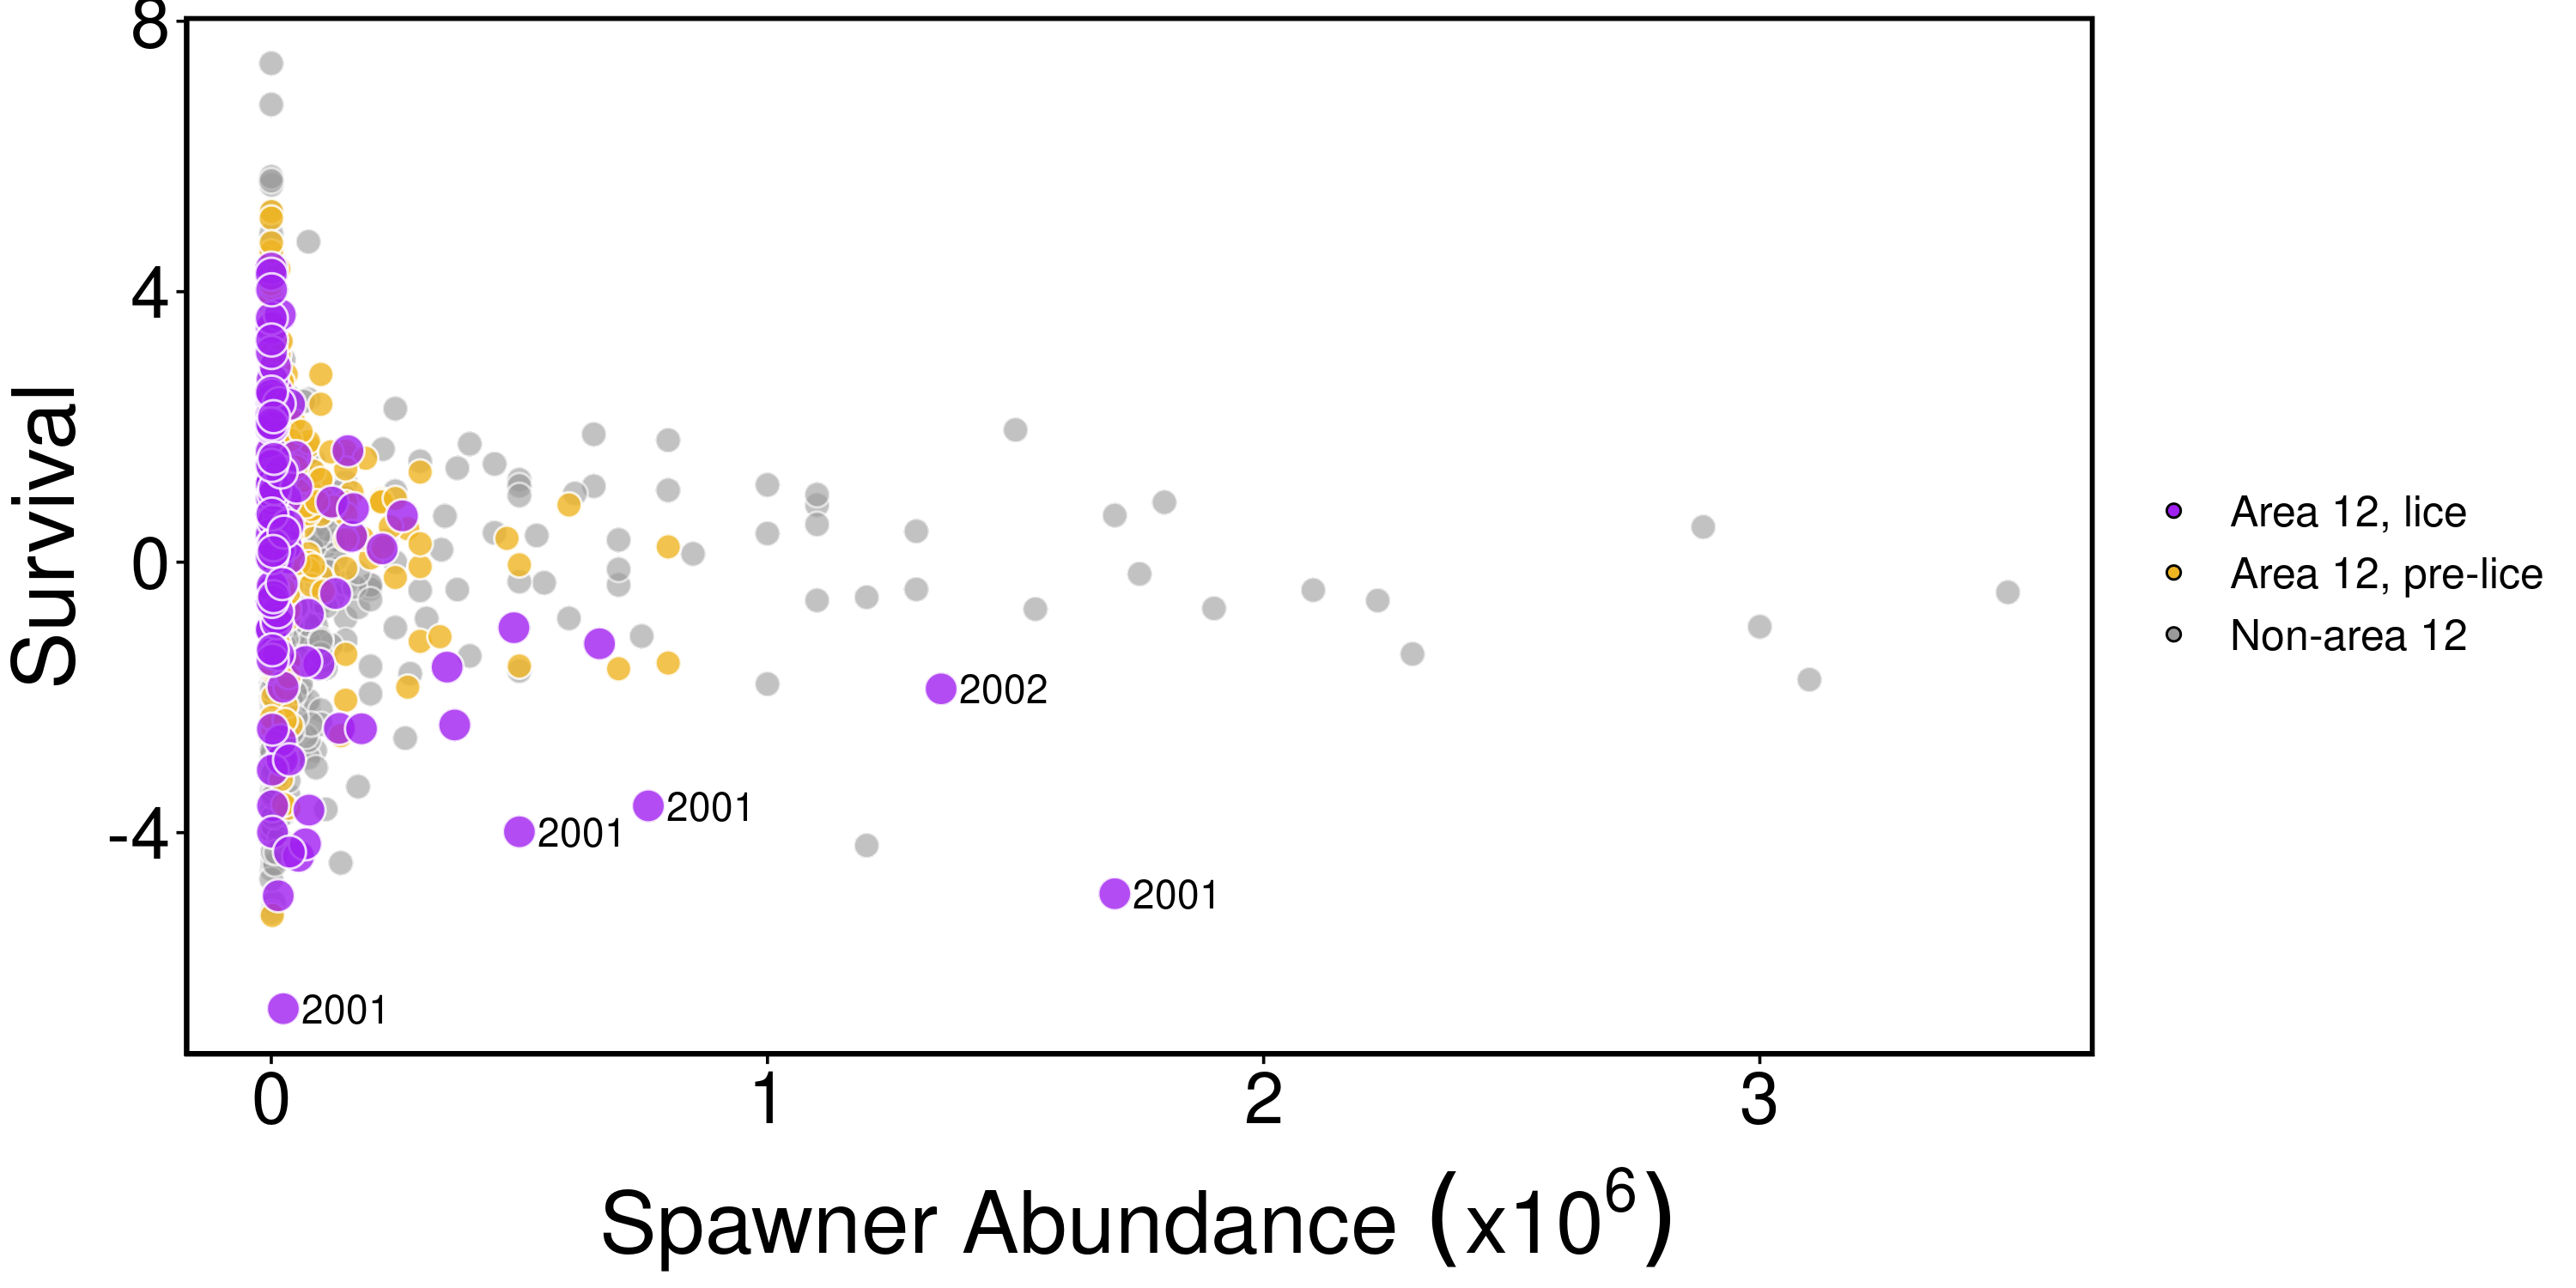
\includegraphics[width=1.4\textwidth]{images/three-classes-of-data.png}}%
    \caption{Survival (log scale) of pink salmon on the y-axis, and spawner abundance on the x-axis. Outlier values with especially low survival but high abundance are labelled.}
    \label{fig:surv}
\end{figure} 

\textbf{Power analysis stuff to go here}

\section{Discussion}

Overall points:
\begin{itemize}
    \item $c$ increased in magnitude even though the years added weren't high estimated \% mortality years 
    \item something about the discrepancy between salmon coast measurements on lice and why that isn't high along with the timeseries data in 2020/2021 (see below for this)
    \item effectiveness of treatment
    \item discuss how using just the KTC farms gave a close correlation but humphrey sargeant doctors didn't
    \item a bunch of space dedicated to sample size and power analysis stuff. 
\end{itemize}

Thoughts on the descrepancy between the number of lice in >2020 in the timeseries plot and the salmon coast estimates:
\begin{itemize}
    \item First and most obvious one is that if you line up the sampling periods with the timeseries you actually might see that they treated in time? I'll have to do this
\end{itemize}

\printbibliography

\end{document}
